\documentclass{article}
\usepackage{amsmath}
\usepackage{listings}
\usepackage{xcolor}
\usepackage{graphicx}
\usepackage{geometry}
\usepackage{hyperref}
\usepackage{tikz}
\usetikzlibrary{trees, positioning}
\geometry{margin=1in}

\title{Hash Tables}
\author{}
\date{}

\definecolor{codegray}{rgb}{0.5,0.5,0.5}
\definecolor{backcolour}{rgb}{0.95,0.95,0.92}

\lstdefinestyle{cppstyle}{
  backgroundcolor=\color{backcolour},
  commentstyle=\color{codegray},
  keywordstyle=\color{blue},
  numberstyle=\tiny\color{codegray},
  stringstyle=\color{red},
  basicstyle=\ttfamily\footnotesize,
  breakatwhitespace=false,
  breaklines=true,
  captionpos=b,
  keepspaces=true,
  numbers=none,
  numbersep=5pt,
  showspaces=false,
  showstringspaces=false,
  showtabs=false,
  tabsize=2,
  language=C++
}

\begin{document}

\maketitle

A \textbf{hash table} is an \textbf{associative data structure} that maps \textbf{keys to values}. Unlike sequential data structures such as arrays or linked lists, which organize elements by position, hash tables provide access to values via arbitrary keys. This allows for efficient average-case performance for \textbf{insertion}, \textbf{deletion}, and \textbf{lookup} operations—typically in $\mathcal{O}(1)$ time.

Hash tables are widely used in compilers, databases, caches, and dictionaries, where fast retrieval by key is critical.

\section{Use Cases}
\begin{itemize}
  \item Implementing associative arrays or maps
  \item Caching computed results (memoization)
\end{itemize}

\section{Time Complexity}
\begin{tabular}{|c|c|c|}
\hline
\textbf{Operation} & \textbf{Average Case} & \textbf{Worst Case} \\
\hline
Insert & $\mathcal{O}(1)$ & $\mathcal{O}(n)$ (with poor hash function or high load) \\
Lookup & $\mathcal{O}(1)$ & $\mathcal{O}(n)$ \\
Update & $\mathcal{O}(1)$ & $\mathcal{O}(n)$ \\
Delete & $\mathcal{O}(1)$ & $\mathcal{O}(n)$ \\
\hline
\end{tabular}

\section{Underlying Implementation}

Hash tables are typically backed by an array. A \textbf{hash function} maps a key to an index in this array:
\[
\texttt{index} = \texttt{hash(key)} \mod \texttt{table\_size}
\]

\subsection*{Example Hash Function (for Strings):}

The following hash function maps a string key to an array index by summing the ASCII values of its characters:

\begin{lstlisting}[style=cppstyle]
int hash(const string& key, int table_size) {
  int sum = 0;
  for (char c : key)
    sum += static_cast<int>(c);
  return sum % table_size;
}
\end{lstlisting}

\textbf{Why use \texttt{\% table\_size}?}

Hash functions often produce large integers. The modulo operation ensures the result is a valid index within the bounds of the underlying array (typically of size \texttt{table\_size}). For example:

\begin{itemize}
  \item If \texttt{sum} = 615 and \texttt{table\_size} = 10, then the index is \texttt{615 \% 10 = 5}.
  \item This maps the key to index 5 in the internal array.
\end{itemize}

This hash function is simple but not collision-resistant. For example:

\begin{itemize}
  \item \texttt{"top"} → ASCII sum = \texttt{116 + 111 + 112 = 339}
  \item \texttt{"pot"} → ASCII sum = \texttt{112 + 111 + 116 = 339}
\end{itemize}

Both strings produce the same hash value:
\[
\texttt{339 \% table\_size} = \texttt{same index}
\]

\textbf{Conclusion:} Anagrams like \texttt{"top"} and \texttt{"pot"} will collide under this hash function. This illustrates the importance of using more sophisticated hash functions that consider character positions and order.

\subsection{Visualizing a Hash Collision}

The diagram below illustrates two different keys mapping to the same index, resulting in a collision:

\begin{center}
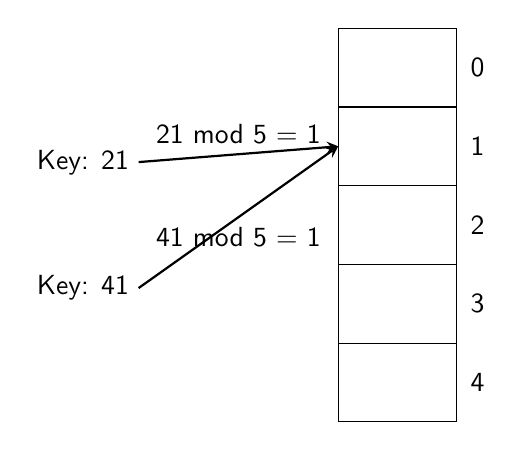
\begin{tikzpicture}[
  table/.style={rectangle,draw,minimum width=1.5cm,minimum height=1cm},
  key/.style={draw,thick,->,>=stealth},
  font=\sffamily
]
% Draw hash table slots
\foreach \i in {0,...,4} {
  \node[table] at (0, -\i) (slot\i) {};
  \node[anchor=west] at (0.8, -\i) {\i};
}

% Draw keys
\node at (-4, -1.2) (k1) {Key: 21};
\node at (-4, -2.8) (k2) {Key: 41};

% Arrows for hashing to same index
\draw[key] (k1.east) -- node[above]{21 mod 5 = 1} (slot1.west);
\draw[key] (k2.east) -- node[below]{41 mod 5 = 1} (slot1.west);

\end{tikzpicture}
\end{center}

\textbf{Observation:} Keys 21 and 41 both hash to index 1, resulting in a collision that must be resolved.

\section{Why Hash Tables Can Perform Poorly}

While hash tables offer average-case constant time, performance degrades in the following scenarios:

\begin{itemize}
  \item \textbf{High Load Factor:} As the number of entries approaches table size, collisions increase and probing chains grow longer.
  \item \textbf{Poor Hash Functions:} If a hash function does not distribute keys uniformly, many values may cluster at the same index.
\end{itemize}

\textbf{Mitigation Strategies:}
\begin{itemize}
  \item Use a well-designed hash function (e.g., MurmurHash, SipHash).
  \item Resize the table dynamically and maintain a low load factor (e.g., below 0.75).
  \item Choose collision resolution wisely (e.g., quadratic probing, double hashing, cuckoo hashing).
\end{itemize}

\section{Collision Resolution Strategies}

Since different keys may hash to the same index (a collision), hash tables use various strategies to resolve them:

\subsection{Chaining (Separate Chaining)}

In separate chaining, each hash table slot holds a pointer to a linked list (or another dynamic structure) of entries that hash to the same index. New entries are appended to the list when collisions occur.

\textbf{Pros:} Simple and flexible; handles collisions gracefully even when the load factor exceeds 1.  
\textbf{Cons:} Requires additional memory for pointers; performance degrades if lists grow too long.

\textbf{C++ STL:} \texttt{unordered\_map} uses separate chaining with buckets internally.

\begin{center}
\begin{tikzpicture}[
  node distance=1.3cm and 1.3cm,
  every node/.style={font=\sffamily},
  table/.style={rectangle, draw, minimum width=1.2cm, minimum height=0.8cm},
  entry/.style={rectangle, draw, minimum width=0.8cm, minimum height=0.6cm},
  arrow/.style={->, thick}
]

% Table slots
\node[table] (slot0) {0};
\node[table, below=of slot0] (slot1) {1};
\node[table, below=of slot1] (slot2) {2};
\node[table, below=of slot2] (slot3) {3};
\node[table, below=of slot3] (slot4) {4};

% Linked list nodes for slot 1
\node[entry, right=of slot1] (n21) {21};
\node[entry, right=of n21] (n41) {41};

% Pointers
\draw[arrow] (slot1) -- (n21);
\draw[arrow] (n21) -- (n41);

% Linked list node for slot 2
\node[entry, right=of slot2] (n37) {37};
\draw[arrow] (slot2) -- (n37);

% Labels
\node[anchor=west] at (3.5, -1.6) {Collision: 21 and 41};

\end{tikzpicture}
\end{center}

\textbf{Explanation:}
\begin{itemize}
  \item Keys 21 and 41 both hash to index 1, forming a linked list.
  \item Key 37 hashes to index 2 and occupies that slot alone.
  \item Each slot acts as the head of a chain.
\end{itemize}

\subsection{Linear Probing}
If a collision occurs at index $i$, search sequentially at $i+1, i+2, \dots$ until an empty slot is found.

\begin{lstlisting}[style=cppstyle]
int probe(int key, int table_size, int i) {
  return (hash(key, table_size) + i) % table_size;
}
\end{lstlisting}

\textbf{Pros:} Simple, good cache performance.  
\textbf{Cons:} Prone to clustering, performance degrades as table fills.

\subsection{Cuckoo Hashing}
Uses two hash functions and two tables. If insertion causes a collision, evict the resident key and relocate it using the other hash function.

\textbf{Pros:} Constant-time worst-case lookup.  
\textbf{Cons:} Complex insertion logic and potential for infinite loops (requiring rehashing).

\subsection{Modern Hash Functions}

Robust hash functions are essential to minimize collisions and ensure uniform distribution:

\begin{itemize}
  \item \texttt{std::hash} (C++ STL): Simple, type-specialized
  \item \textbf{MurmurHash3}: Non-cryptographic, fast and well-distributed
  \item \textbf{CityHash}, \textbf{FarmHash} (Google): Optimized for speed on large inputs
  \item \textbf{SipHash}: Secure hash for short strings; used in Python dictionaries
\end{itemize}

\section{STL \texttt{unordered\_map}}

C++ provides a standard hash table implementation via \texttt{unordered\_map}:

\begin{lstlisting}[style=cppstyle]
#include <unordered_map>
using namespace std;

unordered_map<string, int> freq;
freq["apple"] = 2;
freq["banana"] = 1;
cout << freq["apple"]; // prints 2
\end{lstlisting}

\textbf{Key Characteristics:}
\begin{itemize}
  \item Backed by a hash table
  \item Average $\mathcal{O}(1)$ for insert, find, and erase
  \item Allows custom hash functions via \texttt{std::hash} specializations
\end{itemize}

\section{STL \texttt{unordered\_set}}

The C++ Standard Template Library provides \texttt{std::unordered\_set}, an associative container that stores unique elements using a hash table for fast access.

\subsection{Key Features}

\begin{itemize}
  \item Stores only keys (no associated values)
  \item Ensures uniqueness of elements
  \item Average-case $\mathcal{O}(1)$ time complexity for insert, erase, and find
  \item Backed by hash tables with separate chaining
\end{itemize}

\subsection{Basic Usage}

\begin{lstlisting}[style=cppstyle]
#include <unordered_set>
#include <iostream>
using namespace std;

int main() {
  unordered_set<string> dict;
  dict.insert("apple");
  dict.insert("banana");
  dict.insert("apple"); // duplicate, ignored

  if (dict.find("banana") != dict.end())
    cout << "banana exists\n";

  dict.erase("apple");
}
\end{lstlisting}

\section{Custom Hash Functions}

To use custom types (e.g., structs), you must define both a hash function and an equality comparator:

\begin{lstlisting}[style=cppstyle]
struct Point {
  int x, y;
  bool operator==(const Point& other) const {
    return x == other.x && y == other.y;
  }
};

struct PointHash {
  size_t operator()(const Point& p) const {
    return hash<int>()(p.x) ^ (hash<int>()(p.y) << 1);
  }
};

unordered_set<Point, PointHash> points;
\end{lstlisting}



\section{Practice problem}
Leetcode Problem 1: \textit{Two sum - O(n)}

\url{https://leetcode.com/problems/two-sum/description/}

\end{document}